\documentclass[12pt,a4paper]{article}
\usepackage[utf8]{inputenc}
\usepackage[siunitx,american]{circuitikz}
\usepackage{pgfplots}
\usepackage[margin=0.5in]{geometry}
\usepackage{textcomp}
\usepackage[spanish, es-tabla]{babel}
\usepackage{amsmath}
\usepackage{graphicx}
\usepackage[colorinlistoftodos]{todonotes}
\usepackage{amsmath}
\usepackage{tikz}
\usepackage{booktabs}
\usetikzlibrary{arrows}


\usepackage{parskip}
\usepackage{fancyhdr}
\usepackage{vmargin}
\setmarginsrb{3 cm}{2.5 cm}{3 cm}{2.5 cm}{1 cm}{1.5 cm}{1 cm}{1.5 cm}


\pgfplotsset{compat=1.15}

\begin{document}
\section{Ejercicio 5}


El objetivo de esta sección es implementar un programa en Verilog que multiplique dos números de un digito en formato BCD y expresarlos a la salida como un numero de dos dígitos en formato BCD. Como se trata
de dos números de un dígito en BCD, ambos números serán de 4 bits con un rango de representación de 0 a 9. En cuanto a al producto, como son dos digitos en BCD, seran dos "partes" de 4 bits cada una. 

El primer problema a resolver es el de la multiplicación de dos numeros de 4 bits. Para estudiar el problema se desarrolla dicha operación. La misma se puede ver en la Figura \ref{multiplicacion}. 


\begin{figure}[ht]                                                       
    \centering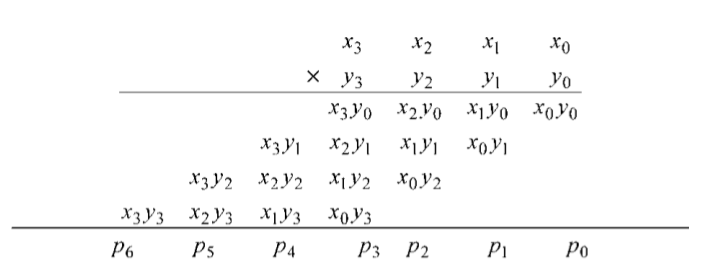
\includegraphics[width=0.8\textwidth, height=5cm]{fig_0.png}
     \caption{Multiplicación de dos números de 4 bits}
     \label{multiplicacion}
     \end{figure}

Como se puede observar se descompuso el producto en $P_0$, $P_1$, $P_2$, $P_3$, $P_4$, $P_5$, $P_6$ y $P_7$. Cada uno de estos bits, que son parte del producto, estan compuestos por sumas de operaciones 
ands y carrys. Por ejemplo: $P_2 = X_1Y_1 + X_0Y_2 + X_2Y_0 + C_in$. Para poder resolver este tipo de operaciones se utilizan circuitos lógicos llamados Half Adder y Full Adder (ver Figura\ref{full_adder}). Ambos circuitos 
lógicos son de gran utilidad. El Half Adder permite hacer sumas de dos bits y devolver su carry. En cuanto al Full Adder, puede sumar (ademas de dos bits) un carry entrante y devolver su respectivo
carry de salida.  Ademas es posible combinar estos circuitos lógicos para obtener distintos resultados.
Volviendo al problema en cuestión, el circuito lógico que devuelve el producto de dos números con dos bits es el que se ve en la Figura \ref{circuito_logico}.


\begin{figure}[h!]                                                       
    \centering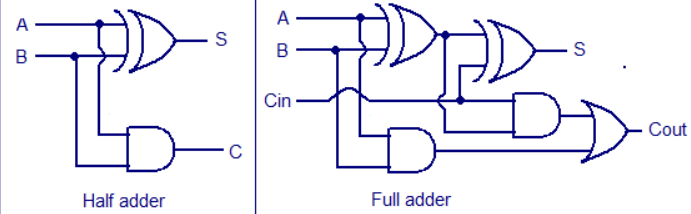
\includegraphics[width=0.8\textwidth, height=4cm]{fig_1.png}
     \caption{Half Adder y Full Adder}
     \label{full_adder}
     \end{figure}



\begin{figure}[h!]                                                       
    \centering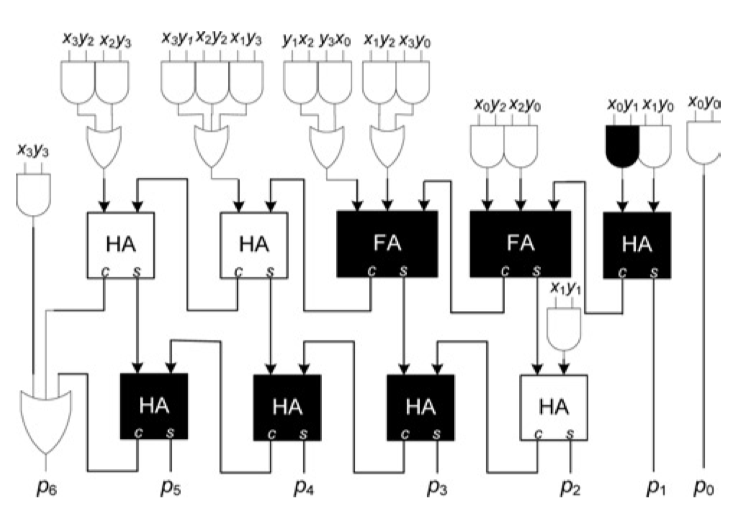
\includegraphics[width=0.8\textwidth]{fig_2.png}
     \caption{Circuito lógico para multiplicar dos números de 4 bits}
     \label{circuito_logico}
     \end{figure}



Como se puede observar el circuito lógico esta compuesto de Half y Full adders. Al tener el diagrama del circuito lógico completo es posible plasmarlo en un script de Verrilog.

Habiendo sobrepasado el inconveniente de obtener el producto de dos números de cuatro bits, surge el problema de convertir dicho numero a BCD. Esto se resuelve fácilmente mediante un algoritmo llamado
Double Dabble. Mediante varias iteraciones del mismo es posible convertir un numero binario en BCD. Para poder utilizar el programa se deben utilizar las siguientes instrucciones: 

\begin{center}
    make\\
    bash run
\end{center}

Estos comandos corren el programa de prueba $ej5\_test.v$ y el programa principal $ej5.v$. 
El programa de prueba somete al programa principal a todas las multiplicaciones posibles para que se devuelva el resultado en BCD.  

\end{document}